\section{Νευρωνικά Δίκτυα με Βάθος}
\label{sec:theory_dnn}

Τα Νευρωνικά Δίκτυα είναι εμπνευσμένα από το βιολογικό νευρικό σύστημα
του ανθρώπου. Η βασική επεξεργαστική μονάδα του εγκεφάλου είναι ο \emph{νευρώνας} (\autoref{fig:neuron_bio}),
ενώ το ανθρώπινο νευρικό σύστημα αποτελείται από περίπου 86 εκατομμύρια νευρώνες και περίπου
$10^14 - 10^15$ διασυνδέσεις.
\begin{figure}[!ht]
  \centering
  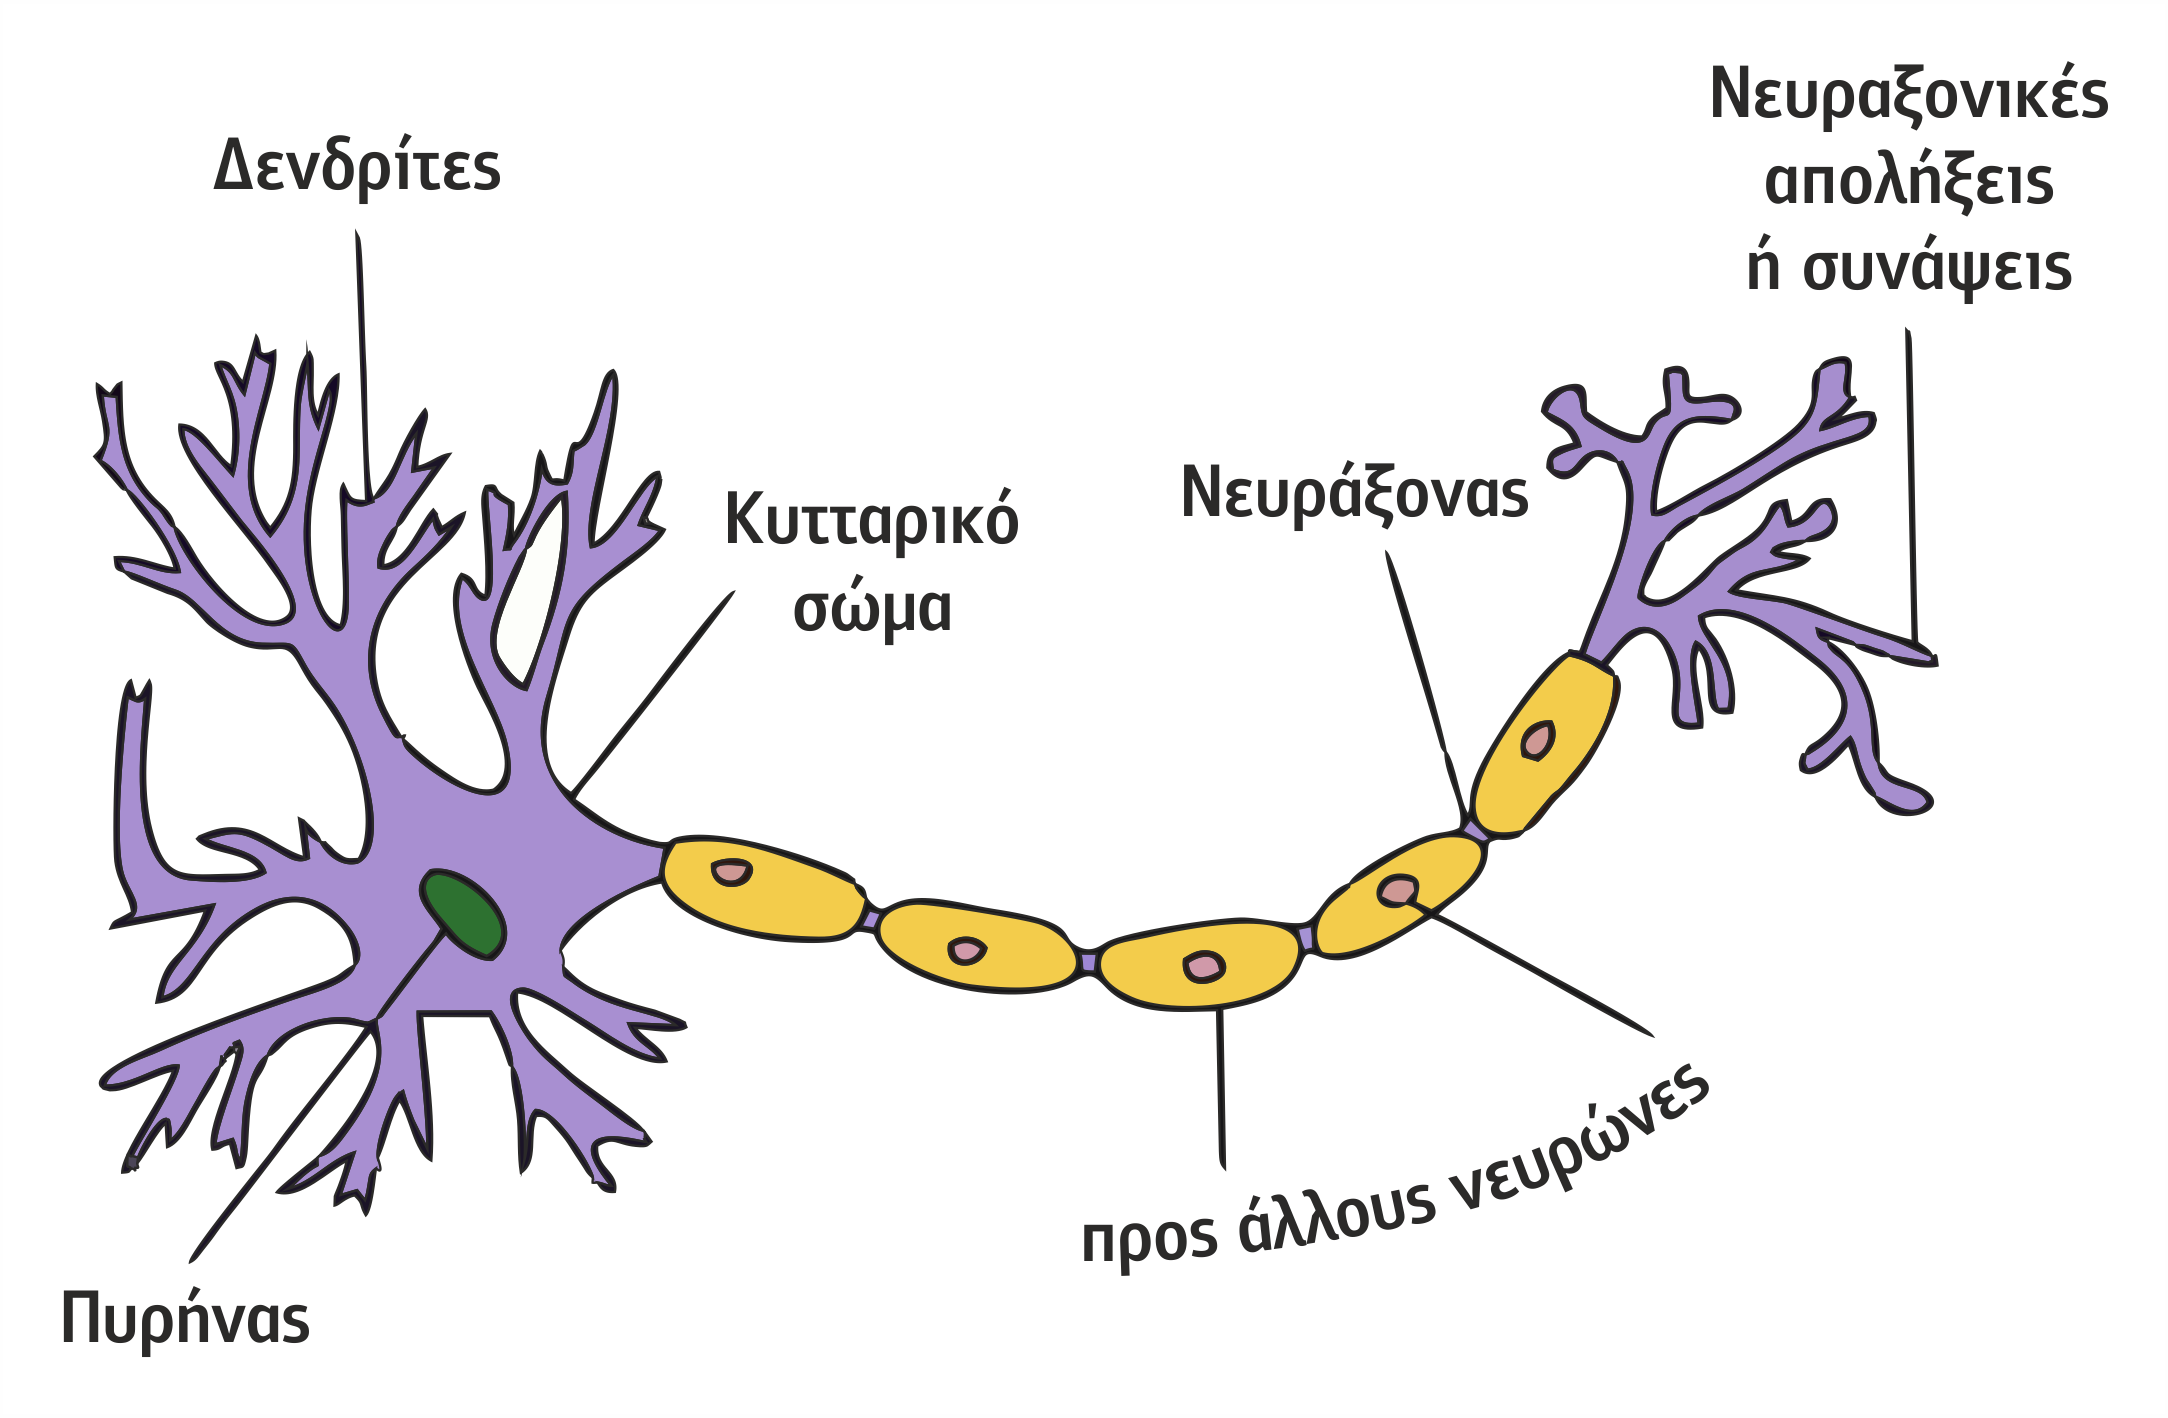
\includegraphics[width=0.7\textwidth]{./images/chapter3/neuron.png}
  \caption[Βιολογικός Νευρώνας]{Βιολογικός νευρώνας.}
  \label{fig:neuron_bio}
\end{figure}
Τα κύρια μέρη ενός νευρώνα είναι τα εξής:
\begin{itemize}
  \item{\textbf{Δενδρίτης (Dendrites)}: Δέχεται είσοδο από άλλους νευρώνες.}
  \item{\textbf{Σώμα του κυττάρου (Cell body)}: Εξάγει συμπεράσματα, με βάση τις εισόδους.}
  \item{\textbf{Νευράξονας (Axon)}: Συνδέει την έξοδο που λαμβάνεται από το σώμα του κυττάρου με τις νευραξoνικές απολήψεις}
  \item{\textbf{Νευραξονικές απολήψεις}: Συνδέει τον νευράξονα του εκάστοτε νευρώνα με τους τερματικούς κόμβους,
    από όπου και μεταφέρεται η πληροφορία στην είσοδο άλλων νευρώνων.}
\end{itemize}
Κάθε νευρώνας δέχεται είσοδο από άλλους νευρώνες μέσω των δενδριτών του και
στην συνέχεια επεξεργάζεται το σήμα που λαμβάνει στην είσοδο και
στέλνει το αποτέλεσμα στον νευράξονα. Τέλος, άλλοι νευρώνες συνδέονται με αυτόν
μέσω των συνάψεων του.

\begin{figure}[!ht]
  \centering
  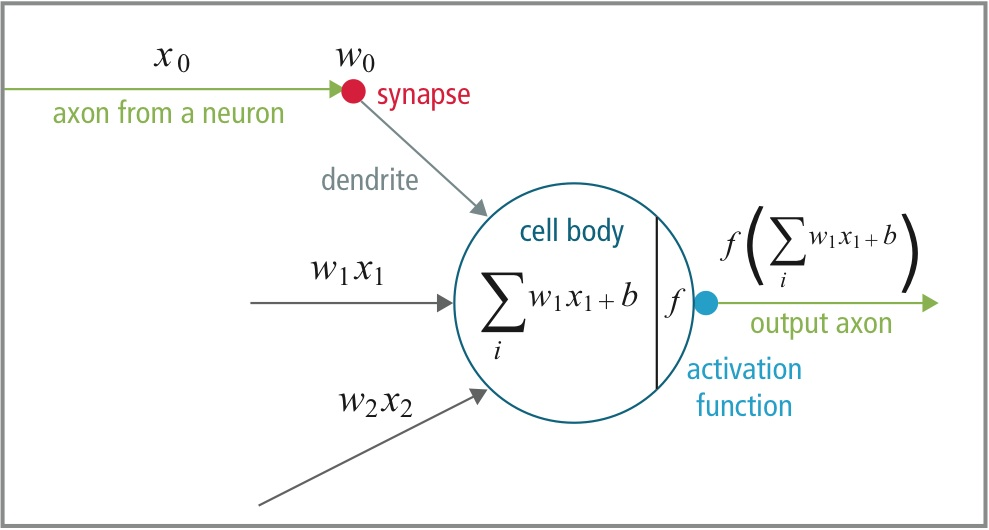
\includegraphics[width=0.7\textwidth]{./images/chapter3/neuron_model.jpg}
  \caption[Μαθηματικό μοντέλο του νευρώνα]{Μαθηματικό μοντέλο του νευρώνα}
  \label{fig:neuron_model}
\end{figure}

Το αντίστοιχο μαθηματικό μοντέλο του νευρώνα, φαίνεται στο \autoref{fig:neuron_model}.
Η πληροφορία που μεταφέρεται από τις νευραξονικές απολήξεις ($x0$), προτού μεταφερθεί
στους δενδρίτες των επόμενων νευρώνων, αλληλεπιδρά πολλαπλασιαστικά με τις
συνάψεις ($w0*x0$). Οι παράγοντες πολλαπλασιασμού $w_n$ ονομάζονται βάρη
και αποτελούν τις μεταβλητές παραμέτρους ενός νευρώνα. Η τιμή των παραμέτρων
αυτών ελέγχει την επίδραση μεταξύ των νευρώνων. Η συνάρτηση ενεργοποίησης $f$
ελέγχει την ροή της πληροφορίας στους συνδεδεμένους νευρώνες
και προσδίδει ευελιξία και ικανότητα εκτίμησης όσον αφορά πολύπλοκες μη γραμμικές
σχέσεις στα δεδομένα εισόδου. Η έξοδος από ένα νευρώνα υπολογίζεται από τη σχέση:
\begin{gather*}
  a = f(\sum_{\imath=0}^{N}w_{\imath}x_{\imath} + b)
\end{gather*}

Η πιο απλή μορφή συνάρτησης ενεργοποίησης
είναι η σιγμοειδής συνάρτηση $\sigma(x) = 1 / (1 + e^{-x})$.
Εναλλακτικά, η σιγμοειδής συνάρτηση ενεργοποίησης μπορεί να εκφραστεί σε διακριτή μορφή ως
\[
f(x) =
  \begin{cases}
    0, & x < 0 \\
    1, & x \geq 0 \\
  \end{cases}
\]
Η επιλογή κατάλληλης συνάρτησης ενεργοποίησης των
νευρώνων δεν είναι τυχαία, αφού όπως θα δούμε στην
συνέχεια επηρεάζει την απόδοση του αλγορίθμου \emph{Backpropagation}, ο οποίος
χρησιμοποιείται για την εκπαίδευση των νευρωνικών δικτύων.

Γενικότερα, ο νευρώνας μπορεί να είναι και πολωμένος (biased - $b$) και έτσι το μαθηματικό
μοντέλο που τον περιγράφει πλήρως παίρνει την μορφή:
\begin{center}
\begin{large}
  $\sigma = f(\sum_{\imath}w_{\imath}x_{\imath} + b) = \frac{1}{1 + e^{-\sum_{\imath}w_{\imath}x_{\imath} + b}}$
\end{large}
\end{center}
Θα μπορούσαμε να ερμηνεύσουμε το αποτέλεσμα της εφαρμογής της
σιγμοειδoύς συνάρτησης ενεργοποίησης ως την πιθανότητα μίας από τις κλάσεις:
%\begin{center}
\begin{large}
\begin{gather*}
  P(y_{\imath} = 1 | x_{\imath};w) \\
  P(y_{\imath} = 0 | x_{\imath};w) = 1 - P(y_{\imath} = 1 | x_{\imath};w)
\end{gather*}
\end{large}
%\end{center}

Σαν παρατήρηση, με εφαρμογή κατάλληλης
συνάρτησης σφάλματος στην έξοδο, ο νευρώνας έχει την συμπεριφορά ενός γραμμικού ταξινομητή
(linear classifier). Πιο συγκεκριμένα, σε περίπτωση που χρησιμοποιήσουμε την \emph{cross-entropy}
συνάρτηση σφάλματος ο νευρώνας μετατρέπεται σε δυαδικό ταξινομητή \textbf{Softmax},
τον οποίο και θα συναντήσουμε στην συνέχεια.

\begin{figure}[!ht]
  \centering
  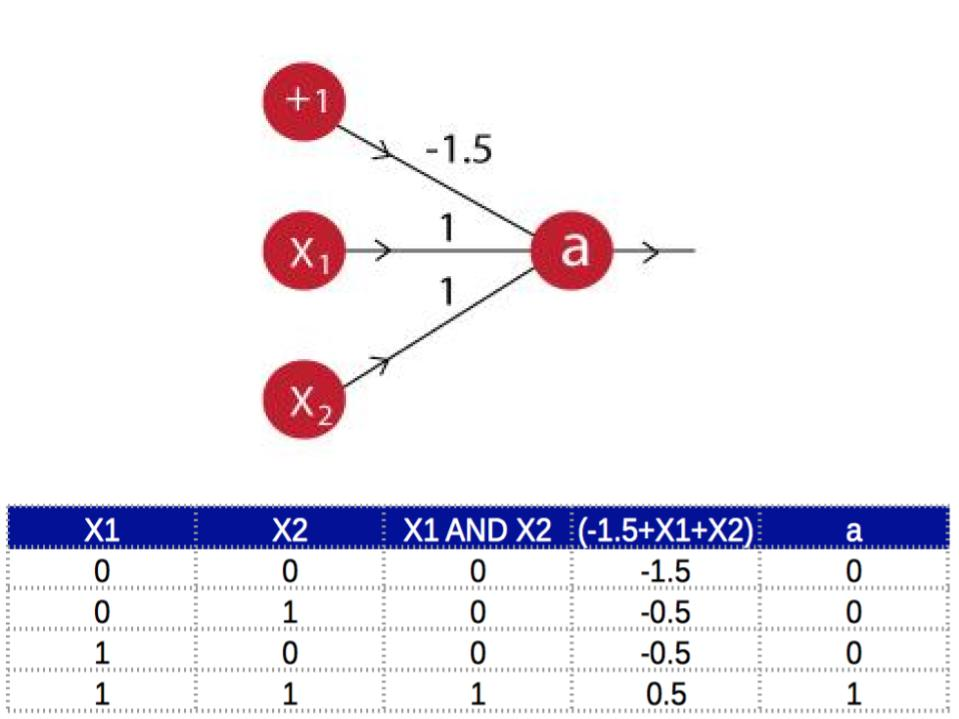
\includegraphics[width=0.6\textwidth]{./images/chapter3/perceptron_and.jpg}
  \caption[Υλοποίηση πύλης AND με χρήση του μαθηματικού μοντέλου του νευρώνα]{Υλοποίηση πύλης AND με χρήση του μαθηματικού μοντέλου του νευρώνα}
  \label{fig:neuron_and}
\end{figure}

Οι τρεις θεμελιώδεις εφαρμογές του μαθηματικού μοντέλου του νευρώνα είναι η
μοντελοποίηση των λογικών πυλών \emph{AND, OR και NOT}. Στο \autoref{fig:neuron_and}
παρουσιάζεται το αντίστοιχο μοντέλο της λογικής πύλης \emph{AND}. Ο νευρώνας
δέχεται σαν είσοδο 2 σήματα ($X_{1}$,  $X_{2}$) και μία παράμετρο πόλωσης ($b=-1.5$).
Η έξοδος $a$ ορίζεται ως:
\begin{gather*}
  a = f(x) = f(X_{1}, X_{2}) =
  \begin{cases}
    0, & x < 0 \\
    1, & x \geq 0 \\
  \end{cases} \\
   x = X_{1} + X_{5} - 1.5
\end{gather*}

Η σύνδεση πολλών νευρώνων σε σε ένα γράφο δομεί ένα \emph{Νευρωνικό Δίκτυο - ΝΝ}.
Το μοντέλο ΝΝ που φαίνεται στο \autoref{fig:simple_nn}
ονομάζεται \emph{Perceptron} ή αλλιώς
\emph{Feedforward Artificial Neural Network - ANN}.
Feedforward γιατί η πληροφορία ρέει προς μία μόνο κατεύθυνση, δηλαδή
η έξοδος νευρώνα στο $\imath$ επίπεδο δεν συνδέεται με την είσοδο νευρώνα
που βρίσκεται το επίπεδο $k \leq \imath$.

Ένα ΑΝΝ έχει τα εξής χαρακτηριστικά:
\begin{itemize}
  \item{Οι διασυνδέσεις μεταξύ των νευρώνων δεν σχηματίζουν σε καμία περίπτωση κύκλο.}
  \item{Αποτελείται από 2 ή περισσότερα κρυφά επίπεδα; ένα κρυφό και το επίπεδο εξόδου}
  \item{Χρησιμοποιείται η σιγμοειδής συνάρτηση ενεργοποίησης}
\end{itemize}

\begin{figure}[!ht]
  \centering
  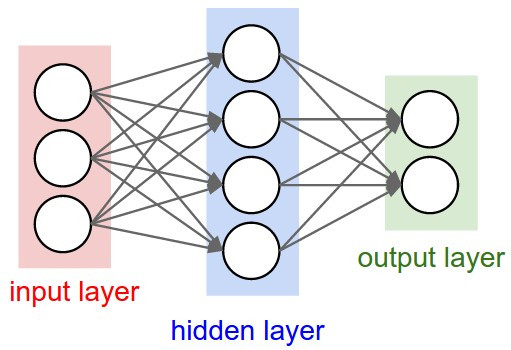
\includegraphics[width=0.5\textwidth]{./images/chapter3/simple_nn.jpg}
  \caption[Απλό μοντέλο NN με ένα κρυφό επίπεδο - Perceptron]{Απλό μοντέλο NN με ένα κρυφό επίπεδο - Perceptron}
  \label{fig:simple_nn}
\end{figure}

To Perceptron δεν είναι το μόνο
μοντέλο ΝΝ που ανήκει στην κατηγορία των Feedforward ANN. Όπως θα δούμε στο
\autoref{sec:theory_cnn}, τα \emph{Νευρωνικά Δίκτυα Συνέλιξης
(Convolutional Neural Networks - CNN)} ανήκουν και αυτά στην κατηγορία αυτή.

Η γενική δομή ενός νευρωνικού δικτύου φαίνεται στο \autoref{fig:multilayer_nn}.
Τα γνωρίσματα ενός τέτοιου, \emph{πολυ-επίπεδου ΝΝ}, είναι τα εξής:
\begin{itemize}
  \item{Αριθμός κρυφών επιπέδων}
  \item{Αριθμός των νευρώνων στο κάθε επίπεδο}
\end{itemize}
Η έξοδος από το εκάστοτε επίπεδο μπορεί να εκφραστεί ως
\[
  A_{\imath+1} = f_{\imath}(A_{\imath} \bullet W_{\imath} + B_{\imath})
\]
όπου ο πίνακας $A_{\imath}$ αναφέρεται στην είσοδο και έχει διαστάσεις $M \times N$,
$W$ είναι ο πίνακας με τα βάρη των νευρώνων του εκάστοτε επιπέδου με διαστάσεις
$K \times M$, και τέλος ο πίνακας $B$ διαστάσεων $K \times N$ αναφέρεται στις
τιμές πόλωσης.
Η τιμή $\imath$ αναφέρεται στον αριθμό του εκάστοτε επιπέδου του ΝΝ.
Ο αριθμός των επιπέδων, ή καλύτερα το μέγιστο μήκος του μονοπατιού που ακολουθεί
η πληροφορία από την είσοδο μέχρι την έξοδο του ΝΝ, ορίζει το \emph{βάθος} ενός ΝΝ.

\begin{figure}[!ht]
  \centering
  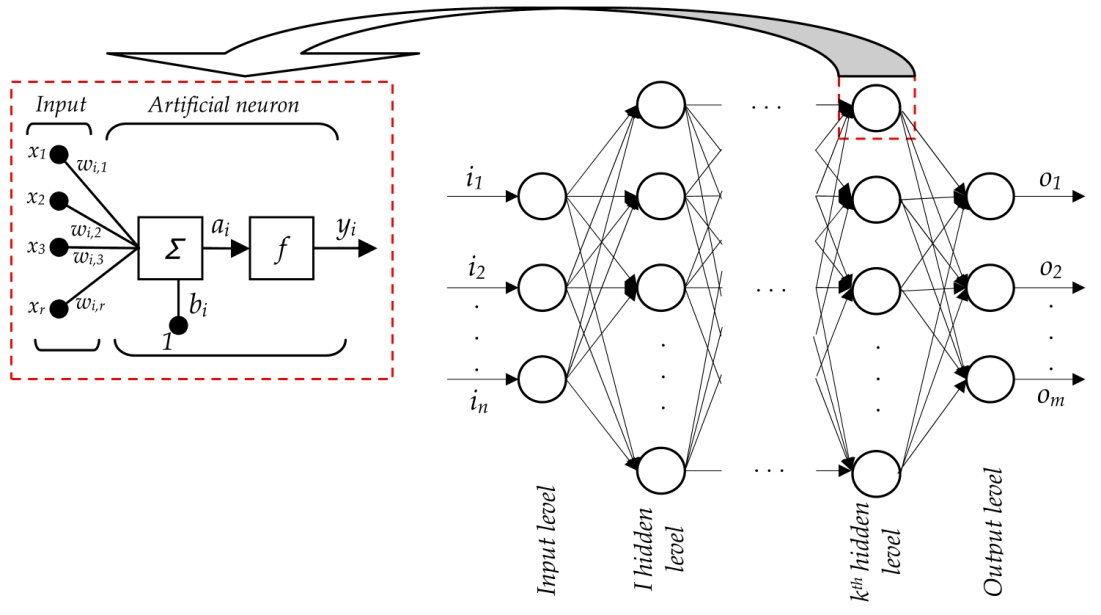
\includegraphics[width=0.9\textwidth]{./images/chapter3/multilayer_nn.jpg}
  \caption[Μορφή ενός πολυεπίπεδου νευρωνικού δικτύου]{Μορφή ενός πολυεπίπεδου νευρωνικού δικτύου}
  \label{fig:multilayer_nn}
\end{figure}

\begin{algorithm}[!htp]
  \caption{Αλγόριθμος Feedforward για τον υπολογισμό των εξόδων ενός επιπέδου του ΝΝ}
  \label{alg:nn_forward}
  \begin{algorithmic}[1]
    \Function{activation}{a}
      \State \Return $1.0 / (1.0 + e^{-a})$
    \EndFunction \\
    \Procedure{nn\_forward}{X, W, B, num\_layers}
      \State Starting from the input layer, use $\sigma$ to do
         a forward pass trough the network, computing the activities of the
        neurons at each layer.
      \State $k \gets 0$
      \While{$k < num\_layers$}
      \State $X^{k} \gets \Call{activation}{X \bullet W_{k} + B_{k}}$  \Comment{If we want to keep output from
        intermediate layers, we must add up one dimension on $X$}.
        \State $k \gets k+1$
      \EndWhile
    \EndProcedure
  \end{algorithmic}
\end{algorithm}

Ο \autoref{alg:nn_forward} υλοποιεί την διαδικασία υπολογισμού της εξόδου
ενός νευρωνικού δικτύου (forward pass), έχοντας σαν δεδομένα τα βάρη και τις τιμές πόλωσης
των νευρώνων του κάθε επιπέδου, καθώς και τα δεδομένα εισόδου.


\subsection{Συναρτήσεις Ενεργοποίησης}

\textbf{Σιγμοειδές - Signmoid}

Η σιγμοειδής μη γραμμική συνάρτηση έχει την μορφή που είδαμε στην αρχή του κεφαλαίου.
Παίρνει σαν είσοδο έναν πραγματικό αριθμό και τον κανονικοποιεί στο διάστημα $[0, 1]$
\[
  \sigma(x) = 1 / (1 + e^{-x})
\]

\begin{figure}[!ht]
  \centering
  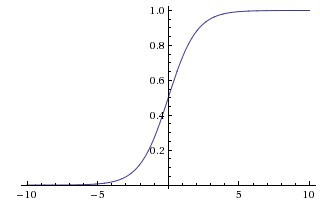
\includegraphics[width=0.4\textwidth]{./images/chapter3/sigmoid.jpg}
  \caption[Συνάρτηση Σιγμοειδούς συνάρτησης]{Συνάρτηση Σιγμοειδούς συνάρτησης}
  \label{fig:sigmoid}
\end{figure}

Πλέον δεν χρησιμοποιείται σε πρακτικές εφαρμογές. Προτιμούνται οι συναρτήσεις
Tanh, ReLU και Maxout.

\textbf{Υπερβολική Εφαπτομένη - Tanh}

Παίρνει σαν είσοδο έναν θετικό αριθμό και τον κανονικοποιεί στο διάστημα $[-1, 1]$
χρησιμοποιώντας την πιο κάτω σχέση:
\[
  \tanh{x} = 2\sigma(2x) - 1
\]

\begin{figure}[!ht]
  \centering
  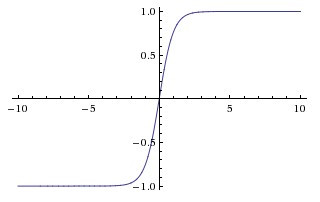
\includegraphics[width=0.4\textwidth]{./images/chapter3/tanh.jpg}
  \caption[Συνάρτηση Υπερβολικής Εφαπτωμένης]{Συνάρτηση Υπερβολικής Εφαπτομένης}
  \label{fig:tanh}
\end{figure}

\textbf{ReLU}

Μία από τις πιο δημοφιλές συναρτήσεις ενεργοποίησης τα τελευταία χρόνια.
Πρακτικά κρατά την ενεργοποίηση οριοθετημένη στο μηδέν και είναι
γρήγορη στον υπολογισμό.
\[
  f(x) = \max(0, x) \equiv f(x) =
  \begin{cases}
    x, \text{Αν} x > 0 \\
    0, \text{Διαφορετικά}
  \end{cases}
\]

\begin{figure}[!ht]
  \centering
  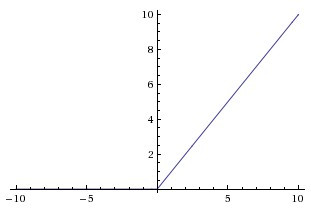
\includegraphics[width=0.4\textwidth]{./images/chapter3/relu.jpg}
  \caption[Συνάρτηση Rectified Linear Unit - ReLU]{Συνάρτηση Rectified Linear Unit - ReLU}
  \label{fig:relu}
\end{figure}

Το μειονέκτημά της είναι ότι κατά την διάρκεια της εκπαίδευσης του νευρωνικού
δικτύου τα βάρη να ανανεώνονται με τέτοιο τρόπο που ο νευρώνας να μην ενεργοποιηθεί
ποτέ. Αυτό έχει σαν αποτέλεσμα να "σκοτώσει" τον εκάστοτε νευρώνα.

\textbf{Leaky ReLU}

Η συνάρτηση ενεργοποίησης Leaky ReLU προσπαθεί να λύσει το προαναφερθέν
πρόβλημα που εμφανίζεται με την χρήση της συνάρτησης ReLU. Αντί να μηδενίζεται
για $x < 0$, η συνάρτηση Leaky ReLU έχει μικρή κλίση:
\begin{equation*}
  f(x) = 1(x<0)(ax) + 1(x\geq0)(x) =
  \begin{cases}
    x, \text{Αν} x>0 \\
    ax, \text{Διαφορετικά}
  \end{cases}
\end{equation*}

\begin{figure}[!ht]
  \centering
  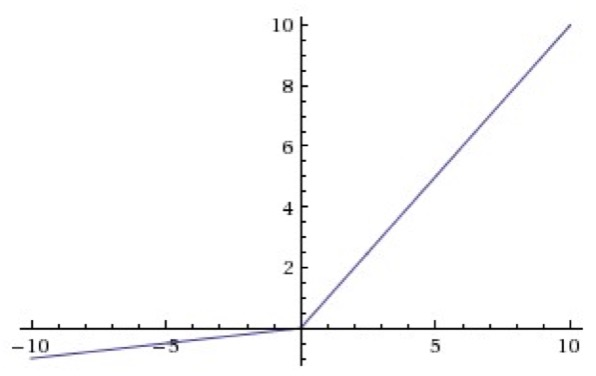
\includegraphics[width=0.4\textwidth]{./images/chapter3/leaky.png}
  \caption[Συνάρτηση Leaky ReLU]{Συνάρτηση Leaky ReLU}
  \label{fig:leaky}
\end{figure}

Η τιμή της σταθεράς $a$ ορίζει την κλίση της συνάρτησης για $x<0$ και μπορεί να δοθεί
σαν παράμετρος του εκάστοτε νευρώνα.

Η πρώτη εφαρμογή της συνάρτησης
Leaky ReLU σαν συνάρτηση ενεργοποίησης νευρώνων έγινε
το 2015 από τον Kaiming He. Οι νευρώνες οι οποίοι χρησιμοποιούν την
συνάρτηση Leaky ReLU ονομάζονται νευρώνες \emph{PReLU} \cite{DBLP:journals/corr/HeZR015}.

\textbf{Maxout}

Η συνάρτηση ενεργοποίησης Maxout \cite{goodfellow2013maxout} είναι η γενίκευση της συνάρτησης Leaky ReLU.
Ένας νευρώνας Maxout, υπολογίζει την συνάρτηση
\begin{equation*}
  f(x) = max(w_{1}x+b_{2}, w_{2}x+b_{2})
\end{equation*}
Παρατηρούμε ότι η πιο πάνω συνάρτηση έχει τέσσερις παραμέτρους
($w_{1}$, $w_{2}$, $b_{1}$ και $b_{2}$). Επίσης, παρατηρούμε οι συναρτήσεις
ReLU και Leaky ReLU είναι ειδικές περιπτώσεις της συνάρτησης Maxout.
Για παράδειγμα, για $w_{1}, b_{1} = 0$ παίρνει την μορφή της συνάρτησης ReLU.
Το μειονέκτημα αυτής της συνάρτησης ενεργοποίησης, σε σχέση με την συνάρτηση
ReLU, είναι ότι διπλασιάζει τις παραμέτρους κάθε νευρώνα.

\begin{figure}[!ht]
  \centering
  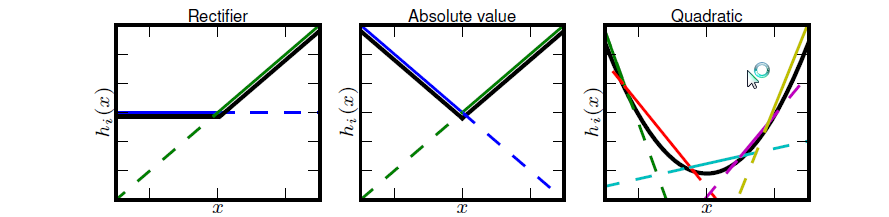
\includegraphics[width=1\textwidth]{./images/chapter3/maxout.png}
  \caption[Συνάρτηση Maxout]{Συνάρτηση Maxout}
  \label{fig:maxout}
\end{figure}

Πρακτικά, τα μοντέλα ΝΝ που χρησιμοποιούν την συνάρτηση Maxout έχουν την
ικανότητα να μάθουν, πέρα από την συσχέτιση μεταξύ των κρυμμένων επιπέδων,
και την συνάρτηση ενεργοποίησης όλων των νευρώνων ενός ή περισσότερων
επιπέδων.
Στο \autoref{fig:maxout} φαίνονται διάφορες μορφές της συνάρτησης Maxout,
μετά από την εκπαίδευση δικτύων Maxout.

\subsection{Συναρτήσεις Σφάλματος/Κόστους}

Είναι κατανοητό ότι τα νευρωνικά δίκτυα χρησιμοποιούνται για την επίλυση
προβλημάτων classification και regression. Γενικότερος στόχος είναι να παρθεί
μία απόφαση, η οποία φαίνεται στην έξοδο του μοντέλου, έχοντας σαν είσοδο
τα δεδομένα του εκάστοτε προβλήματος.
Άρα καταλαβαίνουμε ότι στα μοντέλα ΝΝ τα οποία χρησιμοποιούνται για την επίλυση
τέτοιων προβλημάτων, ενσωματώνεται ένας ταξινομητής (classifier). Ο ταξινομητής
αυτός συνήθως αποτελεί το τελευταίο επίπεδο ενός ΝΝ.

Οι συναρτήσεις σφάλματος έχουν στόχο να τιμωρήσουν τις λανθασμένες αποφάσεις
που λαμβάνονται από τον ταξινομητή, και άρα στην έξοδο ενός ΝΝ,
κατά την διάρκεια της εκπαίδευσης του.

Μία συνάρτηση σφάλματος έχει την γενική μορφή:
\[
  E_{total} = f(target - output)
\]

Σε προβλήματα κατηγοριοποίησης (classification), όπως για παράδειγμα
η αναγνώριση αντικειμένων σε εικόνες, η πιο γνωστή και συχνά χρησιμοποιούμενη συνάρτηση ταξινόμησης
είναι η συνάρτηση \emph{Softmax}, η οποία έχει την μορφή:
\begin{equation*}
  f_{j}(z) = \frac{e^{z_{j}}}{\sum_{k\not=j}e^{z_{k}}} = P(y=\jmath|x)
\end{equation*}
όπου ο δείκτης $j$ αναφέρεται σε ένα στοιχείο του διανύσματος των πιθανών κλάσεων.
Αμέσως καταλαβαίνουμε ότι η πιο πάνω μαθηματική εξίσωση μας δίνει την πιθανότητα
η έξοδος $y$ να ανήκει σε μία εκ του συνόλου των πιθανών κλάσεων, έχοντας
υπό συνθήκη τα δεδομένα εισόδου $x$.
Πιο συγκεκριμένα, παίρνει σαν είσοδο ένα διάνυσμα πραγματικών τιμών ($z$)
και "κατασκευάζει" ένα καινούργιο διάνυσμα του οποίου τα στοιχεία είναι
κανονικοποιημένα στο διάστημα $[0, 1]$ και το άθροισμα τους ισούται με την μονάδα,
δηλαδή $\sum_{k=1}^{N} f_{\jmath}(z) = 1$.

Η συνάρτηση σφάλματος που χρησιμοποιείται στην περίπτωση του ταξινομητή Softmax 
είναι η συνάρτηση \emph{cross-entropy}:
\begin{equation*}
  L_{\imath} = - \log{(\frac{e^{f_{y_{\imath}}}}{\sum_{\jmath}^{} e^{f_{\jmath}}})}
\end{equation*}


Σε προβλήματα regression οι πιο συχνά χρησιμοποιούμενες συναρτήσεις
σφάλματος είναι οι \emph{L1 Norm} και \emph{L2 Norm}.
\begin{gather*}
  L1_{\imath} = \abs{f - y_{\imath}}_{1} \\
  L2_{\imath} = \abs{f - y_{\imath}}^{2}
\end{gather*}
Όπως καταλαβαίνουμε, η πρώτη είναι η συνάρτηση μέσης τιμής ενώ η δεύτερη
είναι η συνάρτηση του τετραγώνου της μέσης τιμής του σφάλματος.

\subsection{Αλγόριθμος Backpropagation}

Ο αλγόριθμος \emph{backpropagation} (\autoref{alg:backpropagation}) εμφανίστηκε το 1970 και υποτιμήθηκε
μέχρι το 1986, όταν και οι David Rumelhart, Geoffrey Hinton, και Ronald Williams
απέδειξαν την αποδοτικότητα του στην εκπαίδευση των νευρωνικών δικτύων, κυρίως
όσον αφορά στην ταχύτητα \cite{rumelhart1988learning}.
Σήμερα ο αλγόριθμος backpropagation χρησιμοποιείται κατά κόρον για την εκπαίδευση
μεγάλων νευρωνικών δικτύων με εκατομμύρια παραμέτρους.

Αυτό που προσπαθεί να καταφέρει ο αλγόριθμος \emph{backpropagation} είναι να
ελαχιστοποιήσει το σφάλμα, δοσμένης μίας συνάρτησης σφάλματος, ορισμένη στον χώρο
των βαρών $w$, χρησιμοποιώντας τον αλγόριθμο \emph{Gradient Descent}.
Υπολογίζει δε το σφάλμα και ανανεώνει ανάλογα τις τιμές του
πολυεπίπεδου νευρωνικού δικτύου, ακολουθώντας μία προς τα πίσω διαδικασία.

Πρακτικά, ο αλγόριθμος backpropagation εφαρμόζει τον κανόνα
της αλυσιδωτής παραγώγισης (gradient chain rule) για τον υπολογισμό των
μερικών παραγώγων, δοσμένης μίας συνάρτησης σφάλματος.

\begin{equation*}
  \frac{\partial z}{\partial x} = \frac{\partial z}{\partial y}\bullet\frac{\partial y}{\partial x}
\end{equation*}

Το πρώτο βήμα για την ελαχιστοποίηση του σφάλματος είναι ο υπολογισμός
της παραγώγου της συνάρτησης σφάλματος ως προς τις παραμέτρους $w$ κάθε επιπέδου,
ή καλύτερα κάθε νευρώνα, του νευρωνικού δικτύου.
\begin{equation*}
  \frac{\partial E_{total}}{\partial w_{ij}}
\end{equation*}

Στο \autoref{fig:backprop} φαίνεται η διαδικασία υπολογισμού της παραγώγου της συνάρτησης
σφάλματος ως προς τις παραμέτρους $w$
ενός νευρωνικού δικτύου που αποτελείται από 1 κρυφό επίπεδο και κάθε επίπεδο
αποτελείται από δύο νευρώνες.

\begin{figure}[!ht]
  \centering
  \hspace*{2cm}
  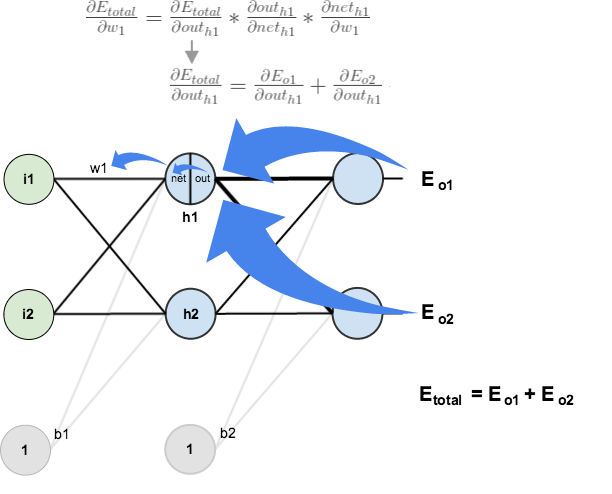
\includegraphics[width=0.6\textwidth]{./images/chapter3/backprop.png}
  \caption[Διαδικασία Backward propagation]{Διαδικασία Backward propagation}
  \label{fig:backprop}
\end{figure}

Η εξίσωση μερικής παραγώγισης της συνάρτησης σφάλματος ως προς την παράμετρο
$w_{1}$ μπορεί να γραφεί σε πιο αναλυτική μορφή:
\begin{gather*}
  \frac{\partial E_{total}}{\partial w_{1}} = (\sum_{k=1}^{O}\frac{\partial E_{total}}{\partial out_{k}}*\frac{\partial out_{k}}{\partial net_{k}}*\frac{\partial net_{k}}{\partial out_{h1}})*\frac{\partial out_{h1}}{\partial net_{h1}}*\frac{\partial net_{h1}}{\partial w_{1}} \\
  \frac{\partial E_{total}}{\partial w_{1}} = (\sum_{k=1}^{O}\delta_{ho}*w_{ho}) * out_{h1}(1-out_{h1}) * i_{1} \\
  \frac{\partial E_{total}}{\partial w_{1}} = \delta_{h1}i_{1}
\end{gather*}
Η αλυσιδωτή παραγώγιση εμπλέκει και την μερική παραγώγιση της
συνάρτησης ενεργοποίησης κάθε νευρώνα ως προς τις παραμέτρους $w$ του.
Άρα καταλαβαίνουμε ότι επιλογή της
συνάρτησης ενεργοποίησης επηρεάζει και την απόδοση, τόσο σε χρόνο εκτέλεσης,
όσο και σε σφάλματα λόγω παραγώγισης, του αλγορίθμου backpropagation.

Η δε ανανέωση των βαρών $w$ γίνεται με βάση την σχέση
\begin{equation*}
  w_{i}^{+} = w_{i} - step * \frac{\partial E_{total}}{\partial w_{i}}
\end{equation*}
δηλαδή αφαιρώντας από την αρχική τιμή την μεταβολή του σφάλματος πολλαπλασιασμένη
με ένα βαθμωτό μέγεθος. Το μέγεθος αυτό οποίο ονομάζεται \emph{ρυθμός ανανέωσης}
των βαρών και είναι σταθερά της διαδικασίας εκπαίδευσης.

Η πλήρης ανάλυση του αλγόριθμου backpropagation ξεφεύγει από τα πλαίσια
της παρούσας διπλωματικής εργασίας. Στην περίπτωση πολυεπίπεδων ΝΝ,
η ανάλυση του γίνεται αρκετά περίπλοκη. Ο αναγνώστης παραπέμπεται στο
κεφάλαιο 6.5 από το βιβλίο \emph{Deep Learning} \cite{Goodfellow-et-al-2016-Book}, όπου και ο αλγόριθμος
\emph{backpropagation} παρουσιάζεται και αναλύεται πλήρως. Πιο συγκεκριμένα,
ο αλγόριθμος 6.1 από το συγκεκριμένο βιβλίο αναφέρεται στην απλή μορφή της διαδικασίας
forward propagation, ο 6.2 είναι μία απλουστευμένη μορφή του αλγορίθμου backpropagation,
ενώ οι αλγόριθμοι 6.3 και 6.4 παρουσιάζουν πλήρως τις διαδικασίες forward και backward
propagation οι οποίοι χρησιμοποιούνται για την εκπαίδευση πολυεπίπεδων νευρωνικών δικτύων,
καταλήγοντας έτσι σε μία ολοκληρωμένη μορφή του αλγορίθμου backpropagation.

\makeatletter
\newcommand{\HEADER}[1]{\State\underline{\textsc{#1}}}
  \newcommand{\ENDHEADER}{}
\makeatother
\newcommand{\STATEI}[1]{\State
  \begin{tabular}{@{}p{\dimexpr \textwidth-\labelwidth}@{}}%
    \hangindent \algorithmicindent
    \hangafter 1
    #1
  \end{tabular}
}

\begin{algorithm}[!htp]
  \caption{Backpropagation learning algorithm}
  \label{alg:backpropagation}
  \begin{algorithmic}
  \For{d in data}
    \HEADER{Forwards Pass}
    \STATEI{Starting from the input layer, do a forward pass trough the network,}
    \STATEI {computing the activities of the neurons at each layer.}
    \ENDHEADER
    \HEADER{Backwards Pass}
    \STATEI{Compute the derivatives of the error function with respect to}
    \STATEI{the output layer activities}
      \For{layer in layers}
      \STATEI{Compute the derivatives of the error function with respect to}
      \STATEI{the inputs of the upper layer neurons}
      \STATEI{Compute the derivatives of the error function with respect to}
      \STATEI{the weights between the outer layer and the layer below}
      \STATEI{Compute the derivatives of the error function with respect}
      \STATEI{to the activities of the layer below}
      \EndFor
      \STATEI{Updates the weights.}
    \ENDHEADER
  \EndFor
  \end{algorithmic}
\end{algorithm}
